\documentclass[11pt]{article}
\usepackage[a4paper,top=3cm,bottom=3cm,left=2.5cm,right=2.5cm]{geometry}
\usepackage[italian]{babel}
\usepackage[utf8x]{inputenc}
\usepackage {caption}
\usepackage {url}
\usepackage {multirow}
\usepackage {booktabs}
\usepackage {fixltx2e}
\usepackage {float}
\usepackage {graphicx}
\usepackage {cite}
\usepackage {listings}
\usepackage {color}
\usepackage {xcolor,colortbl}
\usepackage {adjustbox}
\usepackage {array}
\usepackage {svg}
\usepackage {subfig}
\usepackage {amssymb}
\usepackage {hyperref}
\usepackage {tabulary}
\usepackage {tabularx}
\usepackage[T1]{fontenc}
\usepackage{wasysym}
\usepackage{enumitem}
\usepackage{lipsum}

\newcommand{\voceU}[1]{%
	\item #1\dotfill\Square%
}

\newcommand{\voceD}[1]{%
	\item #1\hfill\Square%
}
\hypersetup{colorlinks=true,citecolor=black,linkcolor=black, urlcolor=blue}

\date{}

\renewcommand{\lstlistingname}{Listato}


\lstset{
    language=C,
    basicstyle=\ttfamily,
    breaklines=true,
    frame=single, % draw a frame at the top and bottom of the code block
    tabsize=2, % tab space width
    showstringspaces=false, % don't mark spaces in strings
    numbers=left, % display line numbers on the left
    captionpos=b,
    commentstyle=\color{green}, % comment color
    keywordstyle=\color{blue}, % keyword color
    stringstyle=\color{red} % string color
}

\begin{document}

\title{\textbf{Definizione ed Implementazione di un Sistema di Raccomandazione Distribuito per film
		e Modellazione di Eventi Complessi}}

\author{\\\textit{Prof. Ing.} Tommaso di Noia\\\textit{Prof.ssa} Marina Mongiello \\
	Mauro Losciale\\ 
	Pietro Tedeschi\\}

\clearpage\maketitle
\thispagestyle{empty}

\begin{center}
	
\includegraphics[scale=0.40]{images/poliba.jpg}
\end{center}

{\textbf{\center Logica e Intelligenza Artificiale\\Ingegneria del Software Avanzata\\ Laurea Magistrale in Ingegneria Informatica\\Politecnico di Bari\\A.A 2015 - 2016\\}}

\newpage
\clearpage
\thispagestyle{empty}
\renewcommand\contentsname{Indice}
\tableofcontents
\newpage
\setcounter{page}{1}

\newpage
\section{Introduzione}
\section{Stato dell'arte}

\subsection{Introduzione ai sistemi CEP}
\subsection{Sistemi di Raccomandazione}
\subsubsection{Filtro collaborativo}
\subsection{Introduzione allo Stream Processing}
\subsubsection{Il paradigma Publish-Subscribe}
\subsection{Il pattern Facade}
\subsection{Il pattern Singleton}
\subsection{Il pattern Model-View-Controller (MVC)}
\subsection{La tecnologia WebSocket}

\section{Analisi del progetto}

\section{Soluzione proposta}

\subsection{La libreria Spark}

Apache Spark è un sistema di cluster computing di tipo general-purpose, scalabile e veloce. Dispone di API di alto livello in \textbf{Java}, \textbf{Scala},\textbf{ Python} ed \textbf{R}, e un engine ottimizzato che supporta grafi di esecuzione generici. Supporta inoltre un ampio set di tool come \textbf{Spark SQL}, per structured data processing, \textbf{MLlib} per il machine learning e \textbf{Spark Streaming}, descritti nelle sezioni successive. Spark è eseguibile sia su sistemi Windows che UNIX-like (Linux, Mac OS). \\

Una delle possibili configurazioni di un sistema Spark è la modalità \textit{cluster}, mostrata in Figura \ref{spark-cluster}. 

\begin{figure}[H]
	\centering
	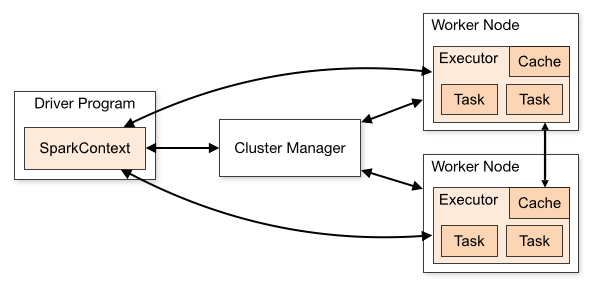
\includegraphics[scale=0.50]{images/cluster-overview.png}
	\caption{Configurazione in Spark di tipo Cluster Mode}
	\label{spark-cluster}
\end{figure}

Le applicazioni Spark sono eseguite come un set di processi indipendenti sul cluster, coordinati dall'oggetto \textit{SparkContext} del programma sorgente (detto \textbf{driver program}). Precisamente, il programma driver può connettersi su diversi tipi di \textit{cluster managers} (ad esempio un cluster di tipo Standalone, Mesos o YARN), il quale alloca le risorse a disposizione delle applicazioni. Una volta connesso, Spark scansiona i nodi del cluster alla ricerca degli \textbf{executor} (detti anche \textit{worker node}), i quali eseguono effettivamente i task e il data storage delle applicazioni. A questo punto il driver invia il codice dell'applicazione agli executor (tipicamente un file JAR o file Python incluso nello SparkContext) e schedula i task per l'esecuzione parallela. 

Alcune considerazioni riguardo tale architettura sono: 
\begin{itemize}
	\item Ogni applicazione gestisce i propri workers, i quali restano attivi durante tutto il ciclo di vita ed eseguono task multipli in thread multipli. Questo implica un isolamento tra le applicazioni, sia lato scheduling (ogni driver schedula i propri tasks) sia lato executor (tasks relativi ad applicazioni differenti risiedono in JVM differenti). Tuttavia ciò implica che non è possibile condividere nativamente i dati tra applicazioni diverse, a meno di utilizzare uno storage system esterno.
	\item Il driver deve poter gestire le connessioni con i workers durante l'intero ciclo di vita dell'applicazione. Per questo motivo dev'essere sempre garantita la visibilità a livello di rete tra driver e workers durante l'esecuzione.
	\item \ `E 
\end{itemize}




\subsubsection{Spark Streaming}

\subsubsection{Spark mllib}
\subsubsection{Spark SQL}

\subsection{Apache Kafka}
\subsubsection{Panoramica}
\subsubsection{Integrazione con Spark Streaming}

\subsection{Il framework Node.js}
\subsubsection{Panoramica}
\subsubsection{Kafka Client per Node.js}
\subsubsection{Il framework Angular.js}
\subsection{La libreria socket.IO}

\section{Conclusioni e sviluppi futuri}

\clearpage
\addcontentsline{toc}{section}{Bibliografia}
\nocite{*}
\bibliographystyle{plain}
\bibliography{biblib}


\end{document}